%\documentclass{article}
%\usepackage{graphicx,subfigure}
%\usepackage{caption,rotating}
%\begin{document}

\begin{figure}[]
\centering
    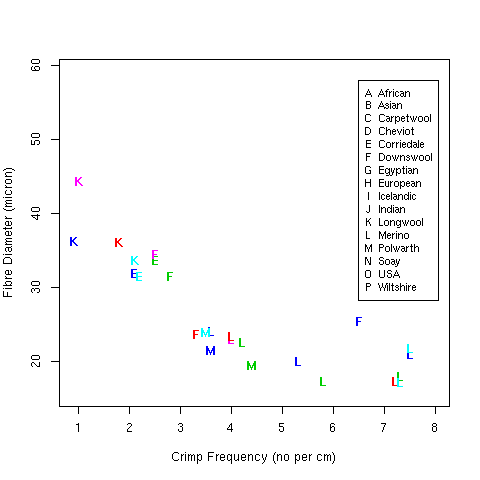
\includegraphics[scale=0.80]{cartercrimpdia.png}
  \caption{Crimp frequency fibre and diameter breed means from Carter(1968)~\cite{carter-1968}. Each point is mean of about 20 sheep from one flock representing a breed.}
\vfill
  \label{fig:cartcrimpdia}
\end{figure}

%\end{document}

